%
% @author   Shmish  "shmish90@gmail.com"
% @legal    MIT     "(c) Christopher Schmitt"
%


\documentclass{article}


%
% Document Imports
%

\usepackage{fancyhdr}
\usepackage{extramarks}
\usepackage{amsmath}
\usepackage{amssymb}
\usepackage{amsthm}
\usepackage{amsfonts}
\usepackage{color}
\usepackage{tikz}
\usepackage{listings}



%
% Document Configuration
%

\newcommand{\hwAuthor}{Christopher K. Schmitt}
\newcommand{\hwSubject}{CS 483}
\newcommand{\hwSection}{Section 01}
\newcommand{\hwSemester}{Fall 2020}
\newcommand{\hwAssignment}{Assignment 2}

\usetikzlibrary{arrows,automata}


%
% Document Environments
%

\setlength{\headheight}{65pt}
\pagestyle{fancy}
\lhead{\hwAuthor}
\rhead{
  \hwSubject \\
  \hwSection \\
  \hwSemester \\
  \hwAssignment
}

\newenvironment{problem}[1]{
  \nobreak\section*{Problem #1}
}{}


%
% Document Start
%

\begin{document}
  \begin{problem}{1}
    \begin{enumerate}
      \item $L_1$ is not regular
      \item $L_2$ is regular, $(0|1)*1(0|1)*1(0|1)*1(0|1)*$
      \item $L_3$ is regular, $(0|1)(00|01|10|11)*$
      \item $L_4$ is regular, $(0)|(1)|(0(0|1)*0)|(1(0|1)*1)$
      \item $L_5$ is not regular
      \item $L_6$ is not regular
    \end{enumerate}
  \end{problem}

  \begin{problem}{2.1}
    \textbf{Theorem:} $L_1$ is not regular.
    \begin{proof}
      Suppose $L_1$ is regular.  Let $p$ be the pumping length given
      by the pumping lemma.\\
      Because any valid arithemtic exression requires balanced
      parenthesis, there must be an equal number of opening and
      closing parenthesis.  We use this to show that $L_1$ is
      not regular.\\
      Choose $s$ to be $o^pc^p$, where $o$ corresponds to the
      opening parenthesis and $c$ corresponds to the closing
      parenthesis.\\
      By the pumping lemma, $s = xyz$ and $xy^iz \in L_1$, for
      any $i \ge 0$.\\
      Because $|xy| \le p$, $x$ and $y$ must all be opening
      parenthesis.\\
      This leads to a contradiction, Because $y \ne \epsilon$ and
      $xy^0z \notin L_1$.  Thus the lemma is broken.
    \end{proof}
  \end{problem}

  \begin{problem}{2.2}
    \textbf{Theorem:} $L_5$ is not regular.
    \begin{proof}
      Suppose $L_5$ is regular.  Let $p$ be the pumping length given by the
      pumping lemma.\\
      Choose $s$ to be $0^p110^p$.\\
      By the pumping lemma, $s = xyz$ and $xy^iz \in L_1$, for any $i \ge 0$.\\
      $|xy| \le p$, so $xy$ must contain only zeros.\\
      By the pumping lemma, $xz \in L_5$, But $xz$ cannot be a palindrome if $i \ge 1$
      given that $y \ne \epsilon$ (x must contain at least one more zero than z).
    \end{proof}
  \end{problem}

  \begin{problem}{2.3}
    \textbf{Theorem:} $L_6$ is not regular.
    \begin{proof}
      Suppose $L_6$ is regular.  Let $p$ be the pumping length given by the
      pumping lemma\\
      Choose $s$ to be $0^p1^p$.\\
      By the pumping lemma, $s = xyz$ and $xy^iz \in L_6$, for
      any $i \ge 0$.\\
      $y$ cannot be $\epsilon$ and $|xy| \le p$, so $y$ only contains zeros.\\
      The pumping lemma says that $xy^2z \in L_6$, but $xy^2z$ contains more
      zeros than ones, and therefore cannot be in $L_6$.
    \end{proof}
  \end{problem}

  \begin{problem}{3}
    \begin{enumerate}
      \item[$L_1$] \begin{tabular}{rl}
        & $S \to a \mid (S) \mid S + S \mid S - S \mid S * S \mid S \div S$
      \end{tabular}

      \item[$L_2$] \begin{tabular}{rl}
        & $S \to T1T1T1T$\\
        & $T \to \epsilon \mid 0T \mid 1T$
      \end{tabular}

      \item[$L_3$] \begin{tabular}{rl}
        & $S \to 0T \mid 1T$\\
        & $T \to \epsilon \mid 0S \mid 1S$
      \end{tabular}

      \item[$L_4$] \begin{tabular}{rl}
        & $S \to 0T0 \mid 1T1 \mid 0 \mid 1$\\
        & $T \to \epsilon \mid 0T \mid 1T$
      \end{tabular}

      \item[$L_5$] \begin{tabular}{rl}
        & $S \to \epsilon \mid 0S0 \mid 1S1 \mid 0 \mid 1$
      \end{tabular}

      \item[$L_6$] \begin{tabular}{rl}
        & $S \to \epsilon \mid SS \mid 0S1 \mid 1S0$
      \end{tabular}
    \end{enumerate}
  \end{problem}

  \begin{problem}{4}
    \begin{center}
      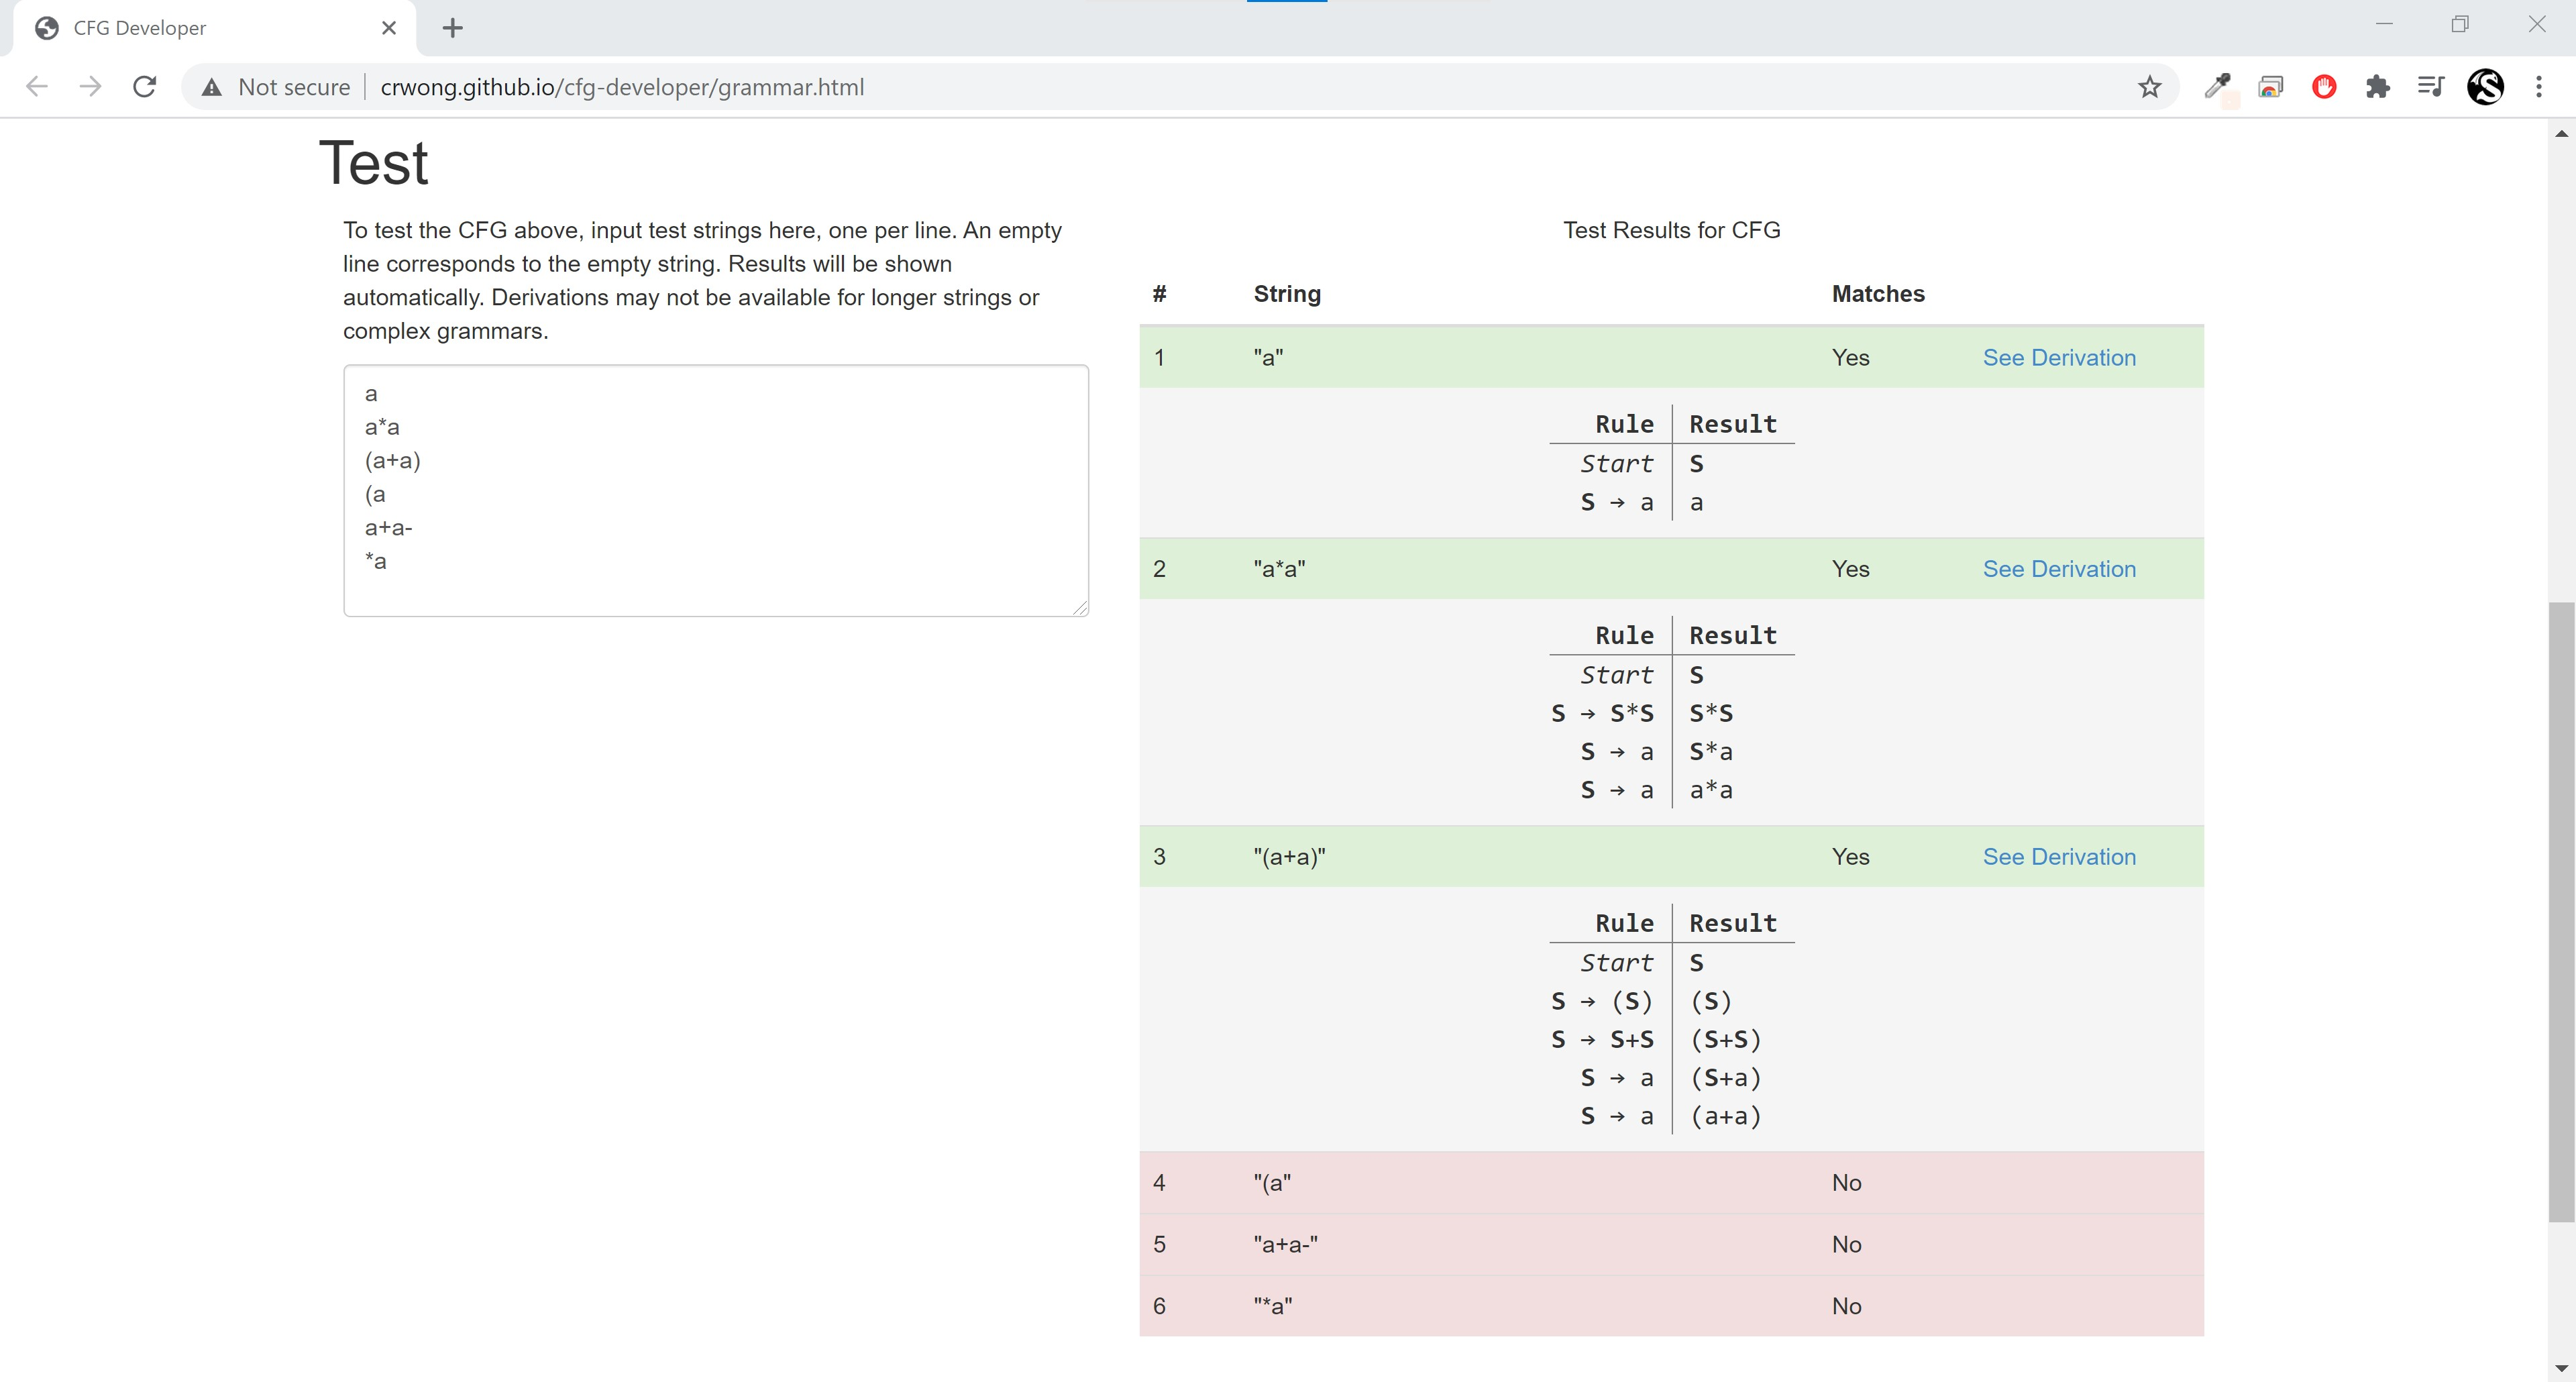
\includegraphics[scale=0.298]{images/L1.jpg}
      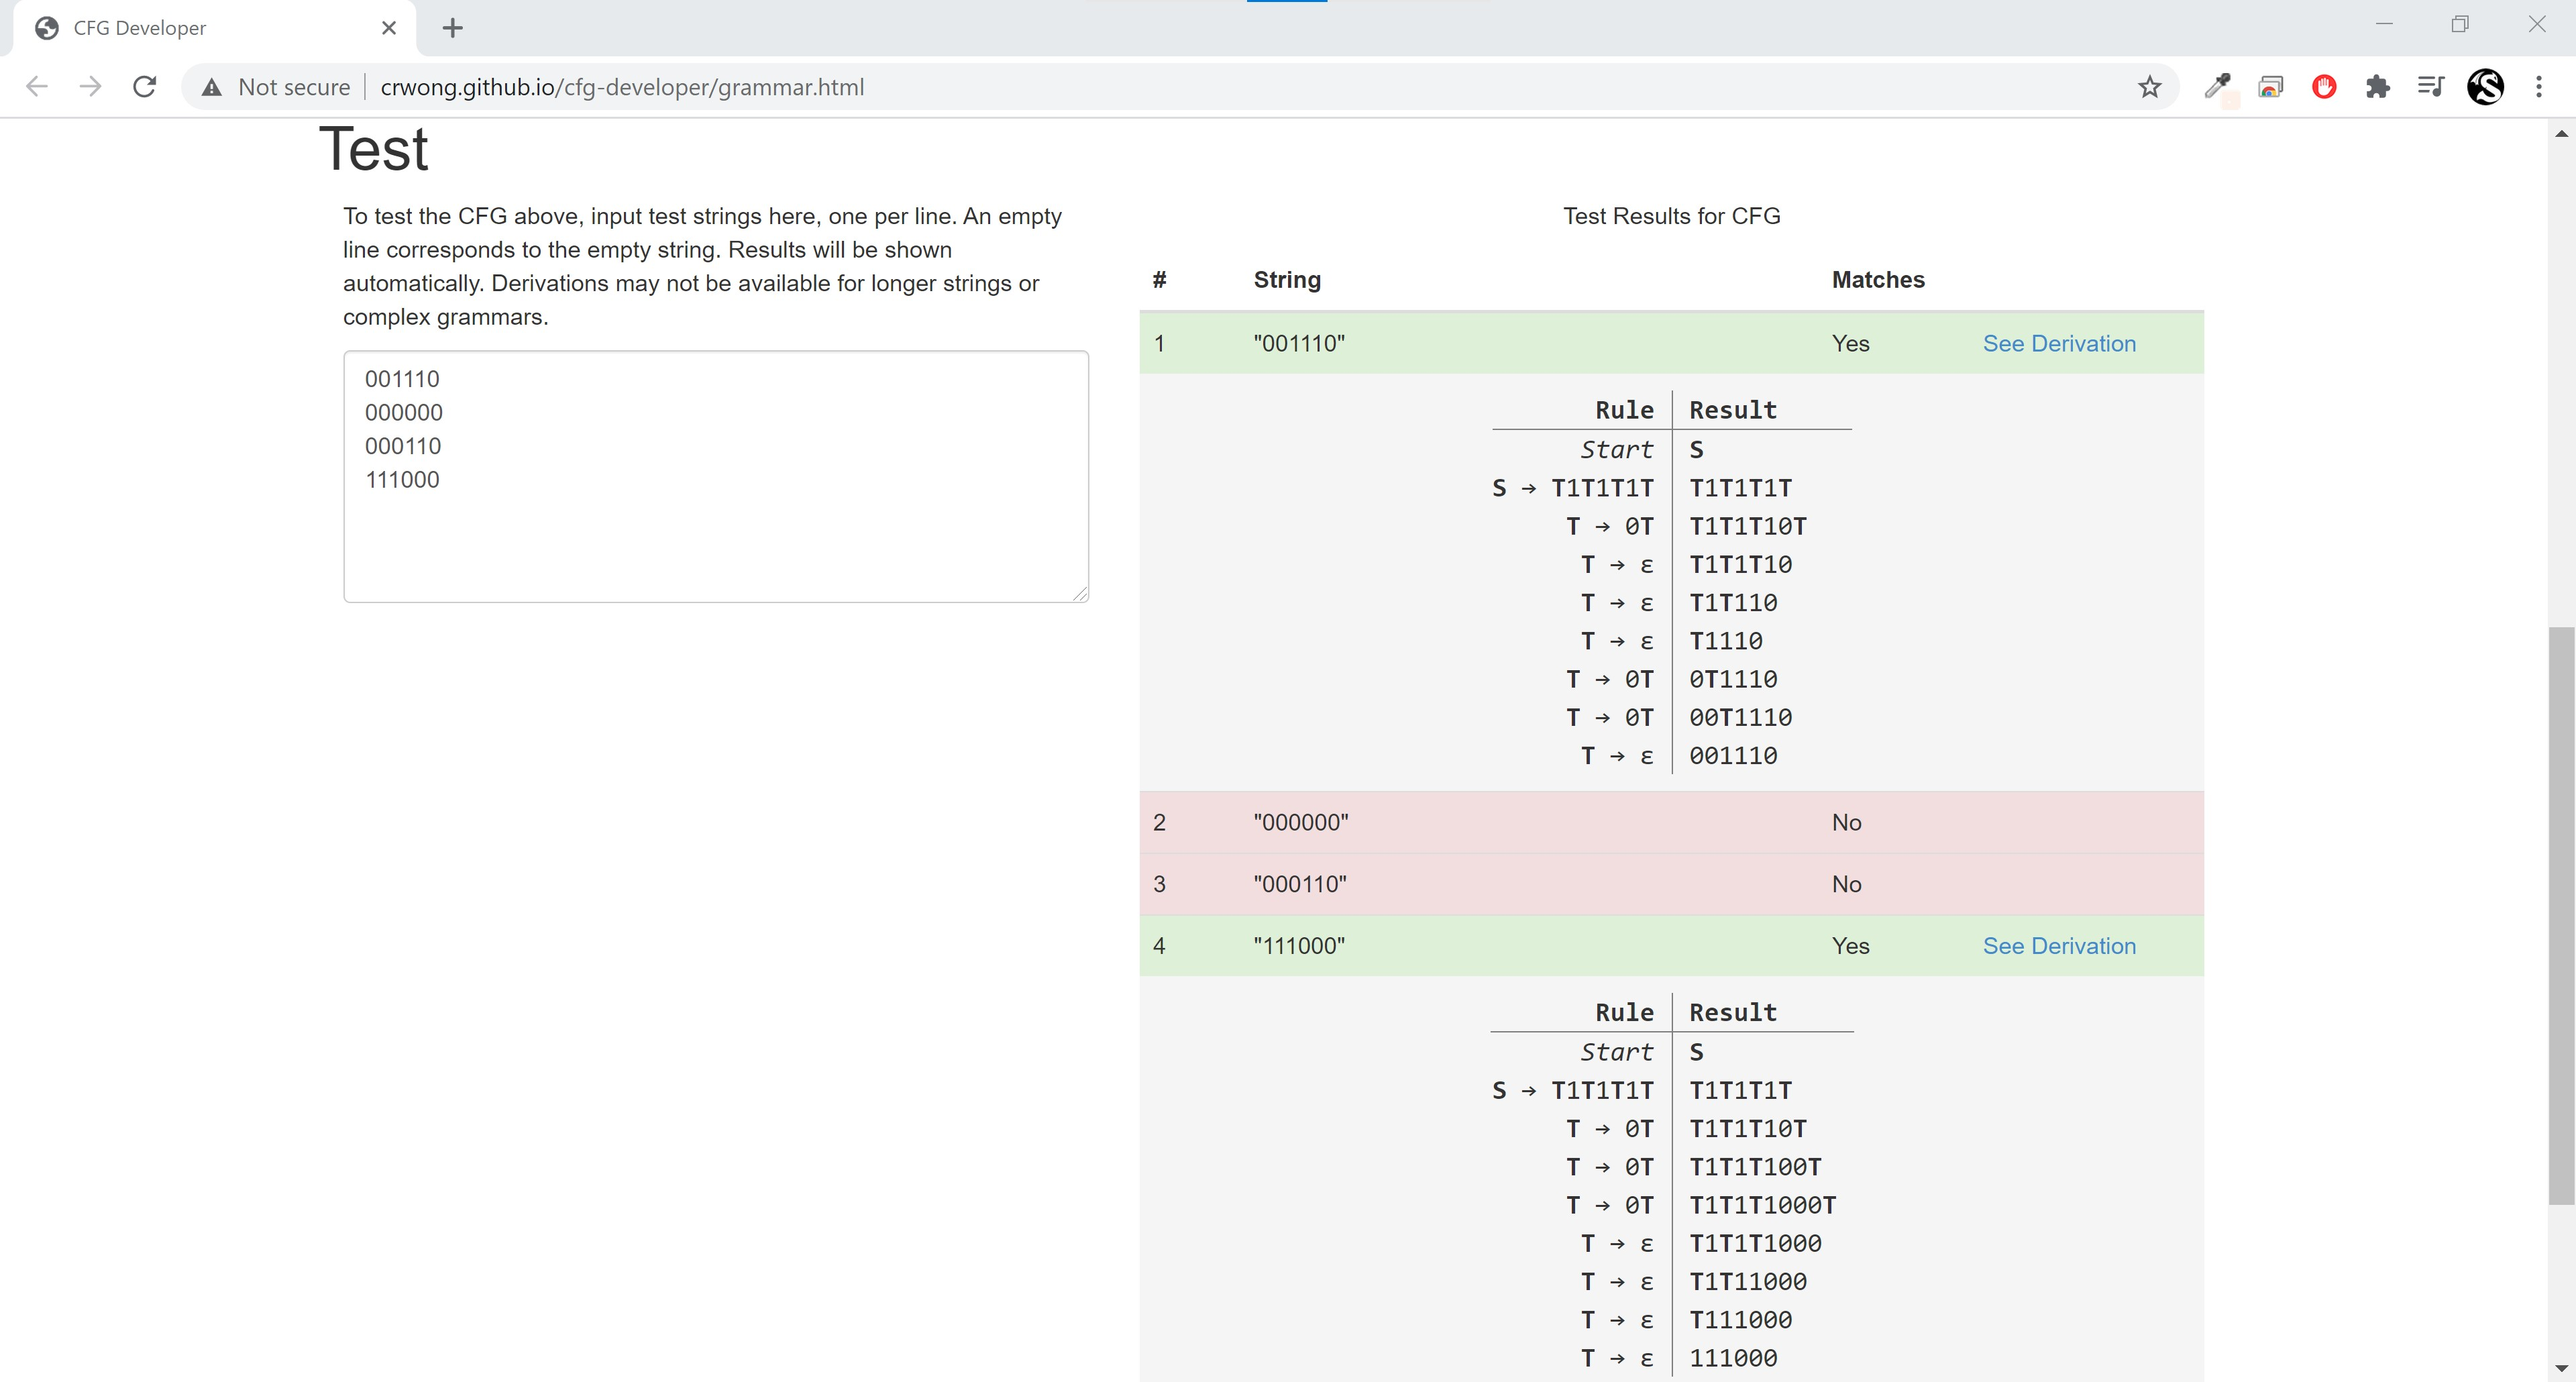
\includegraphics[scale=0.298]{images/L2.jpg}
      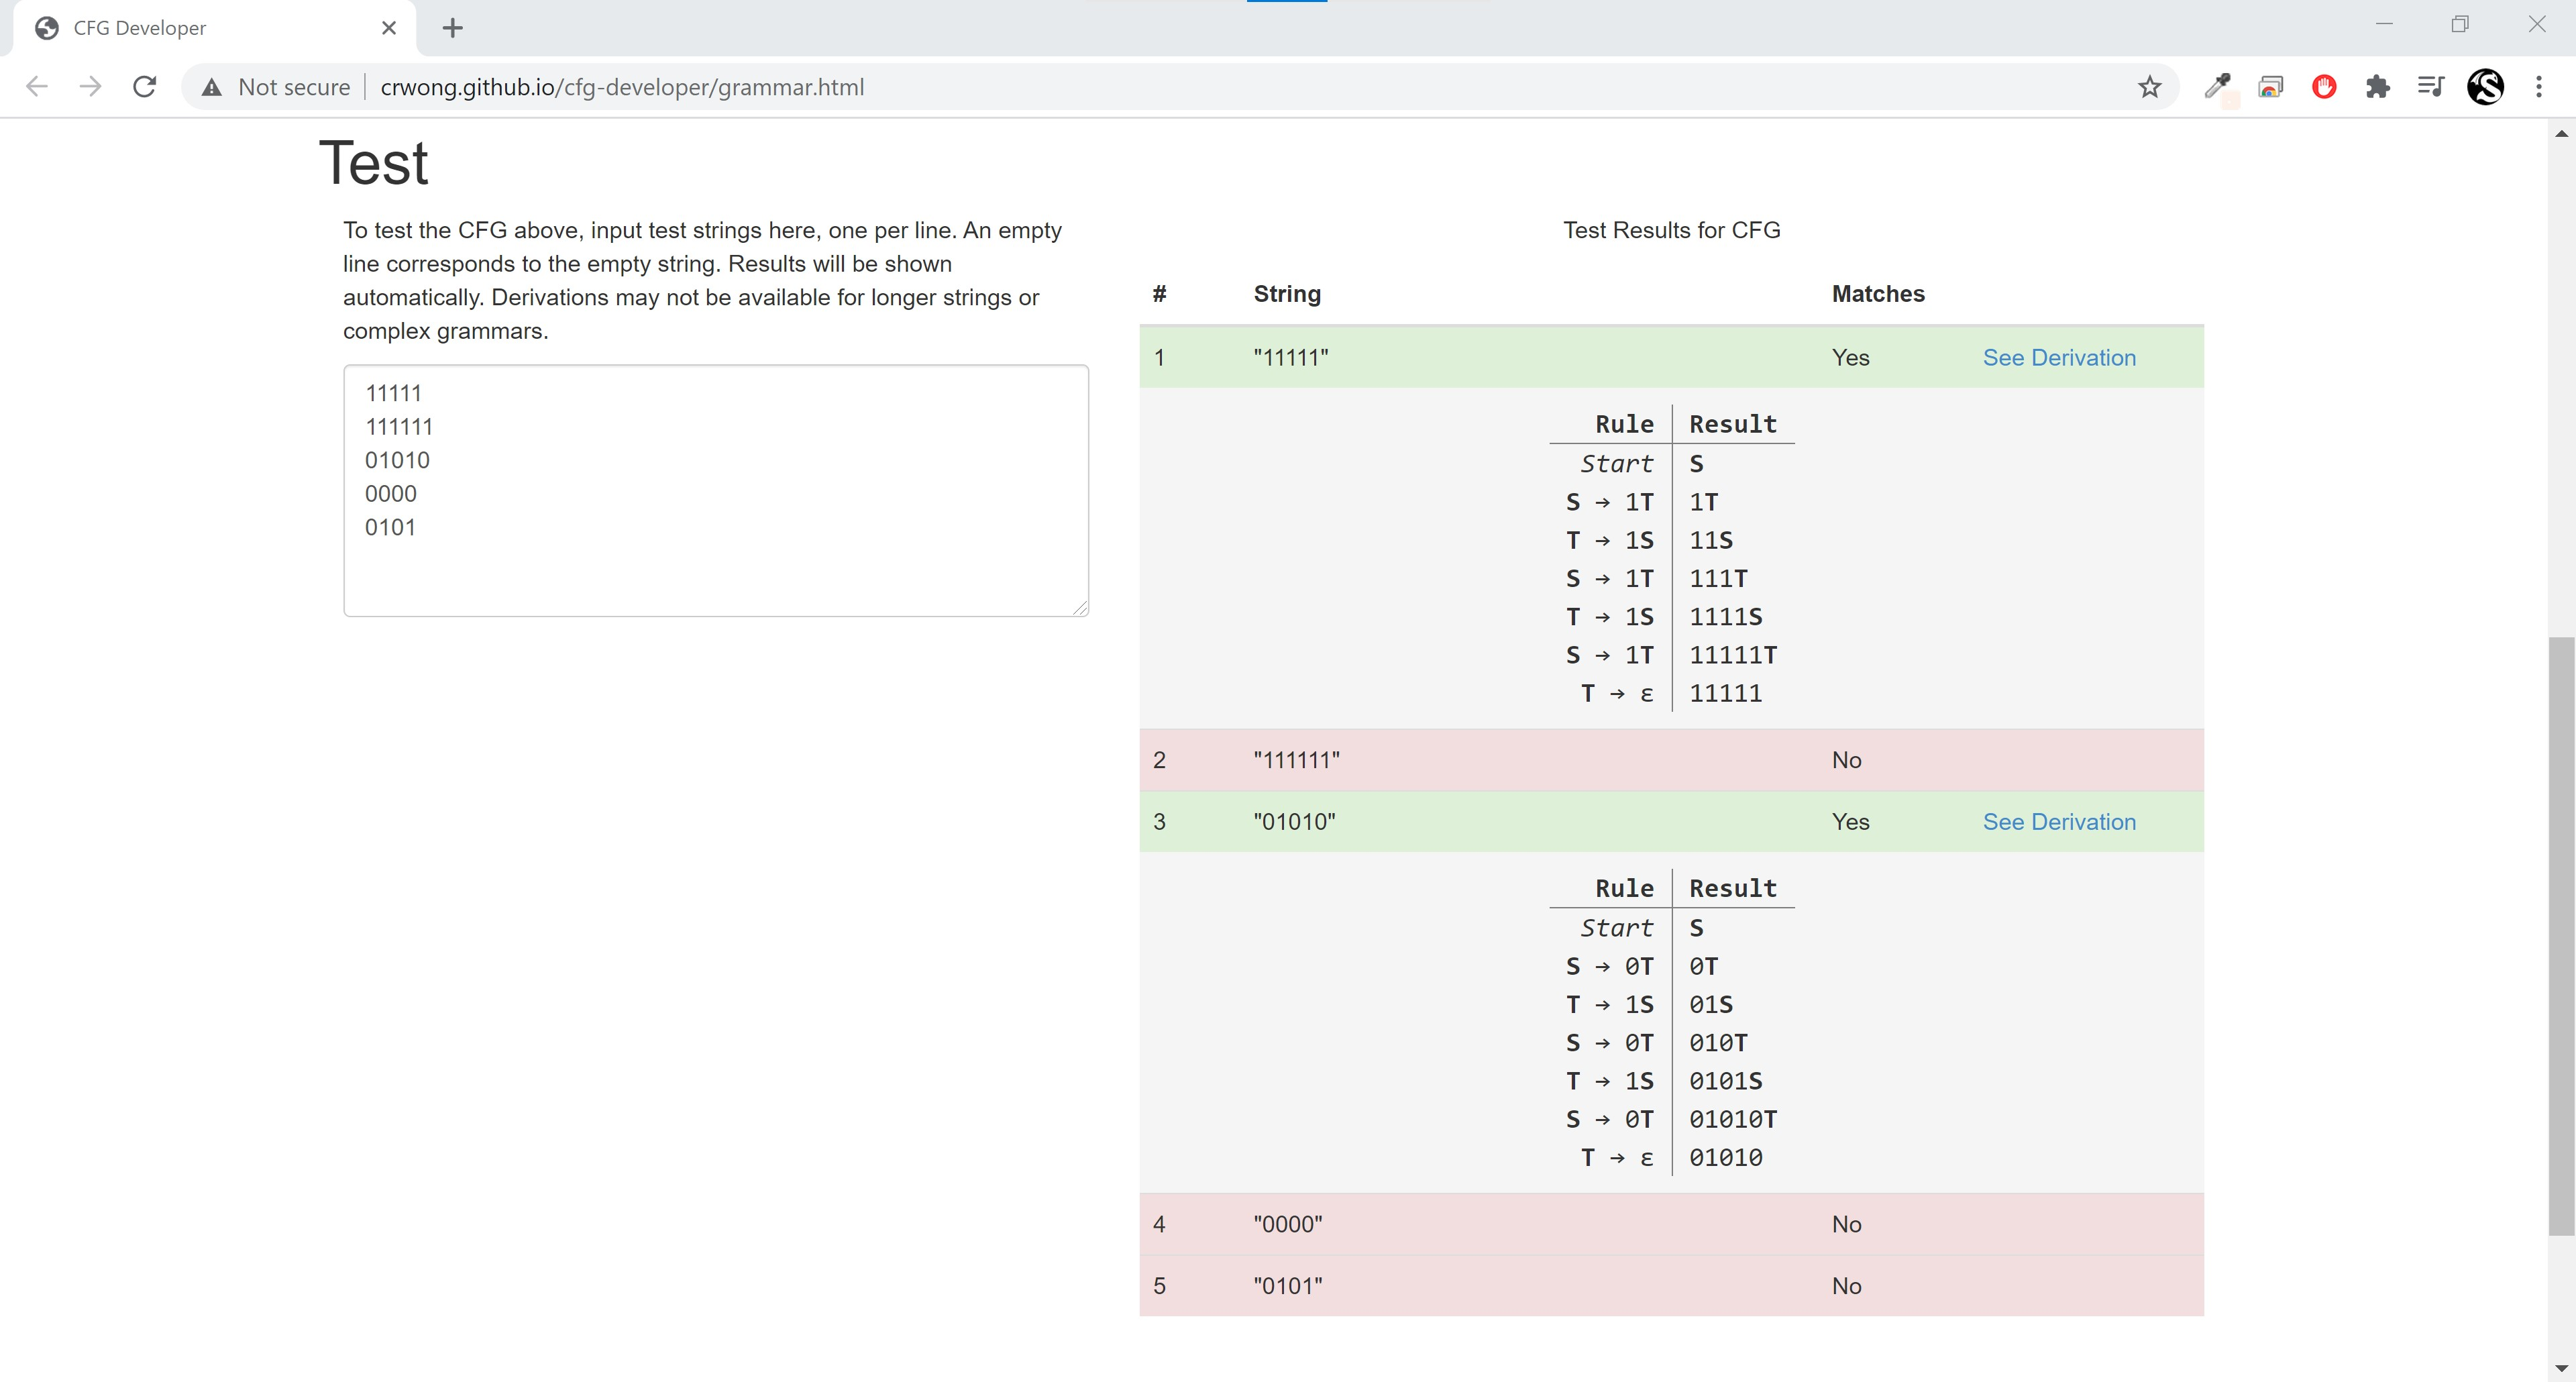
\includegraphics[scale=0.298]{images/L3.jpg}
      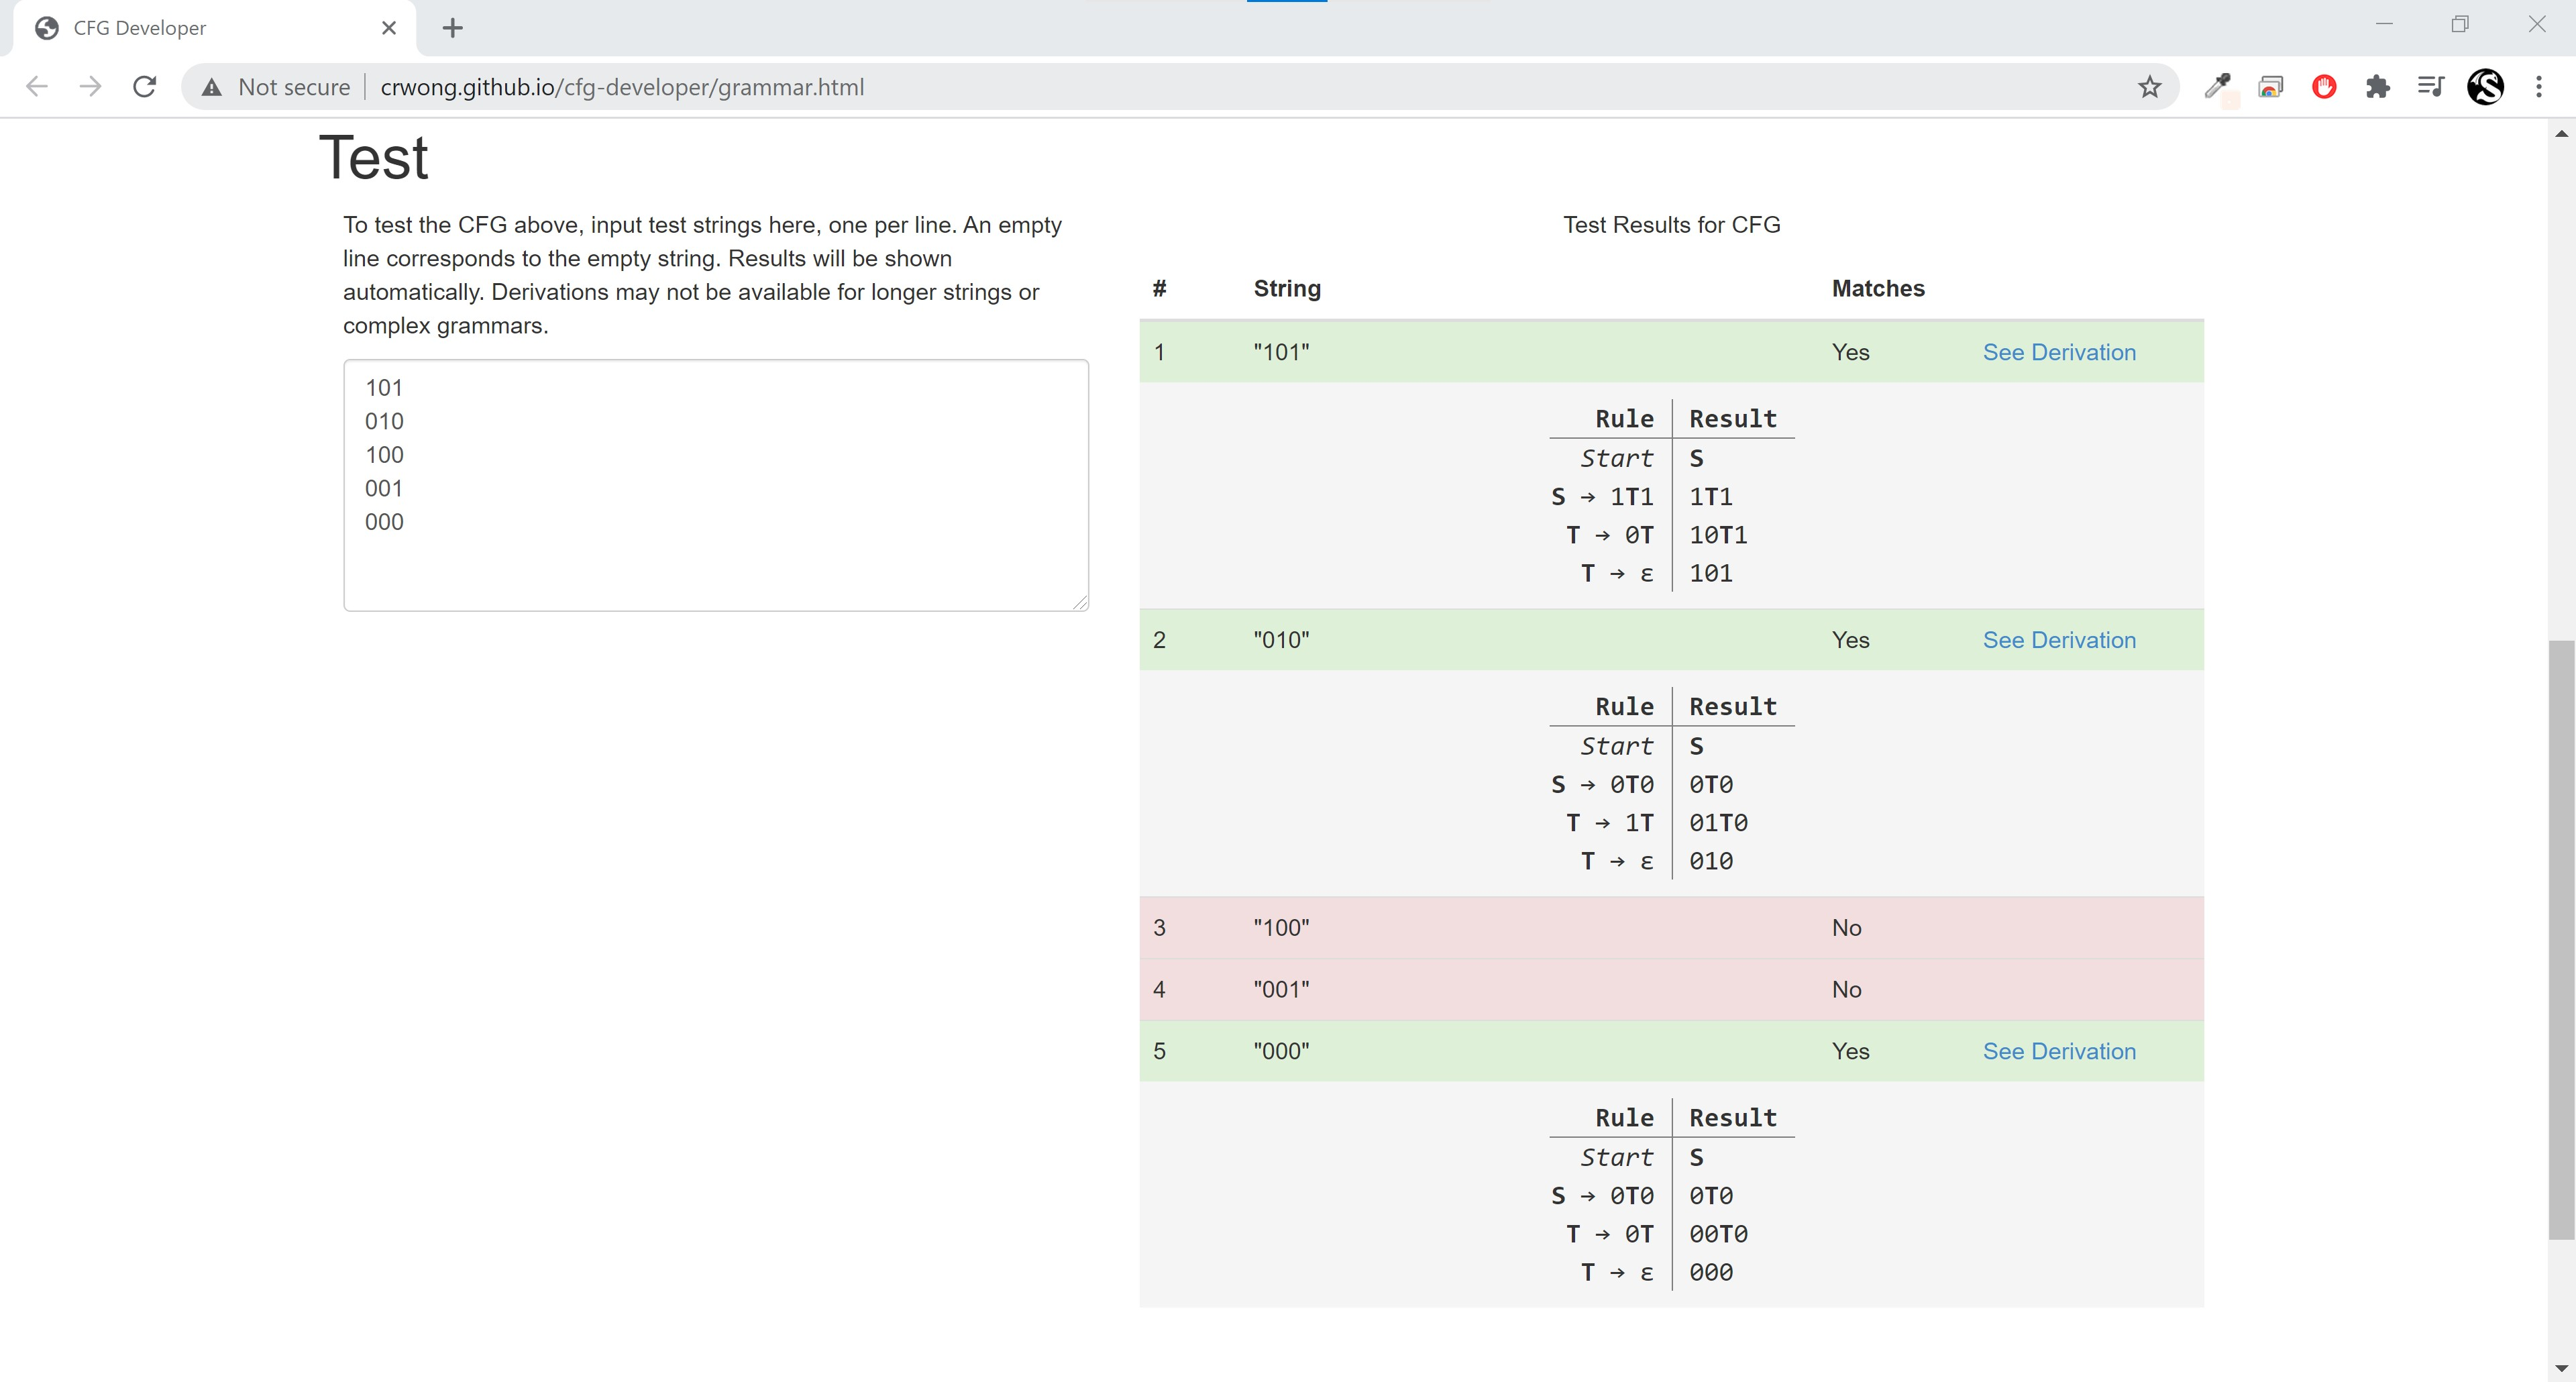
\includegraphics[scale=0.298]{images/L4.jpg}
      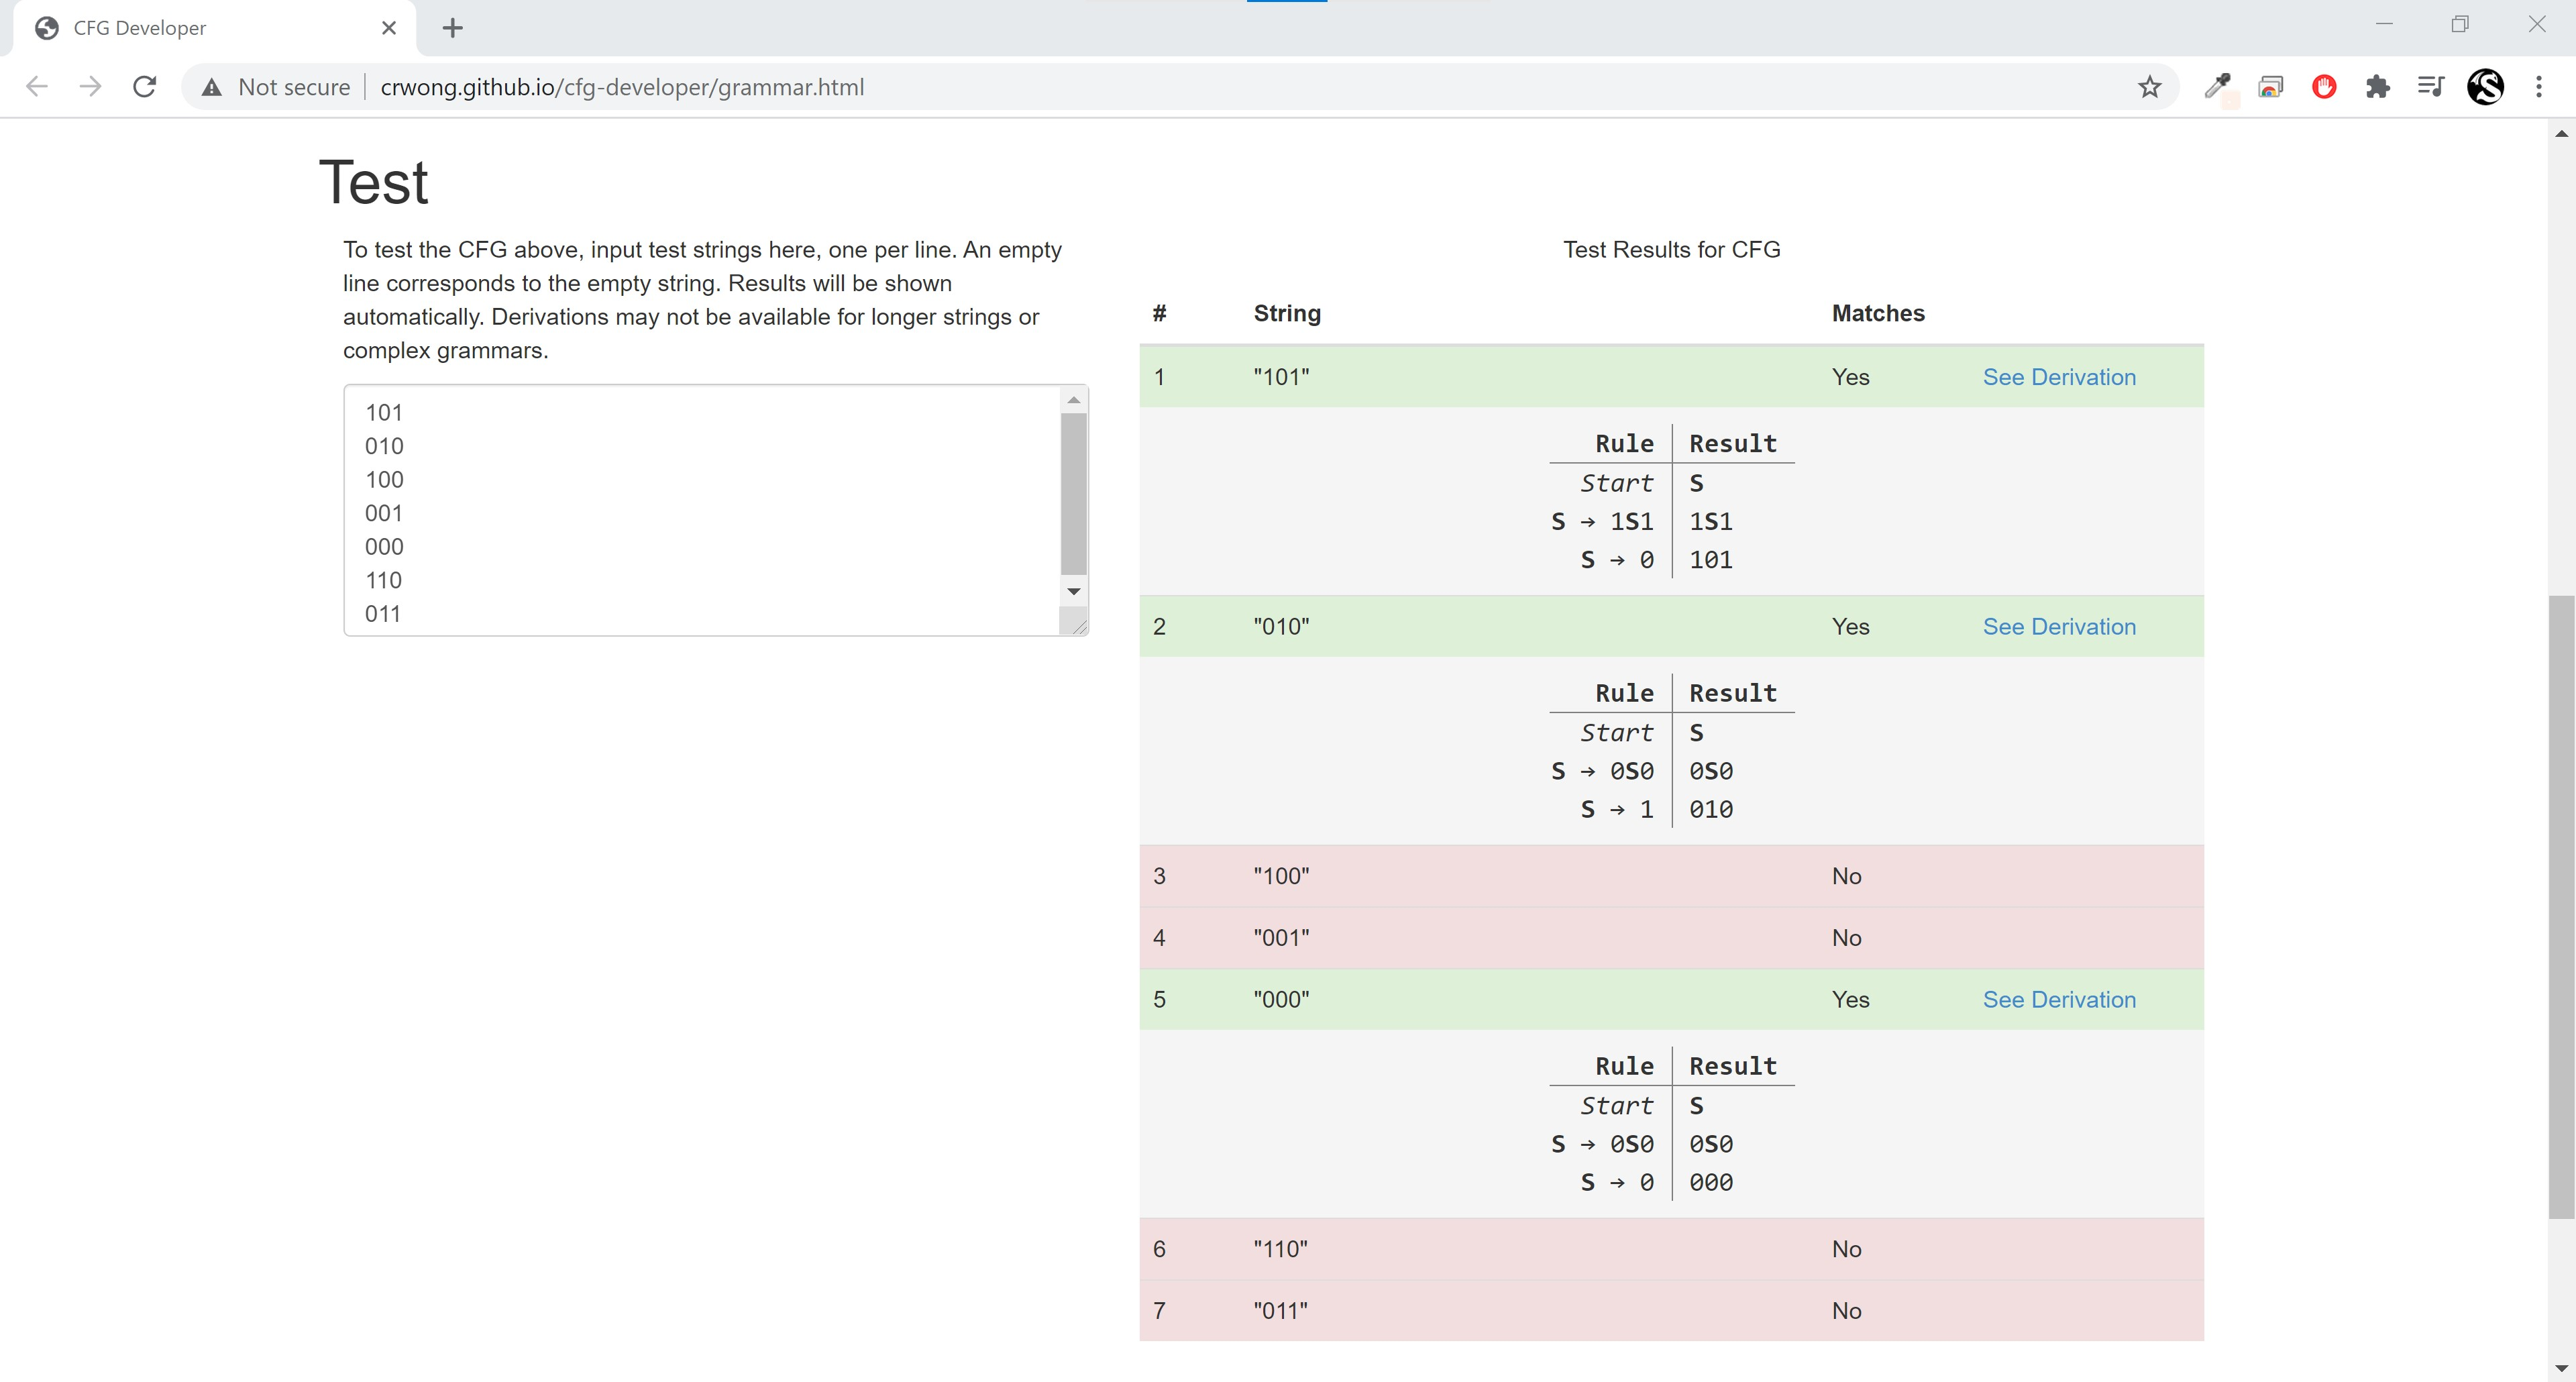
\includegraphics[scale=0.298]{images/L5.jpg}
      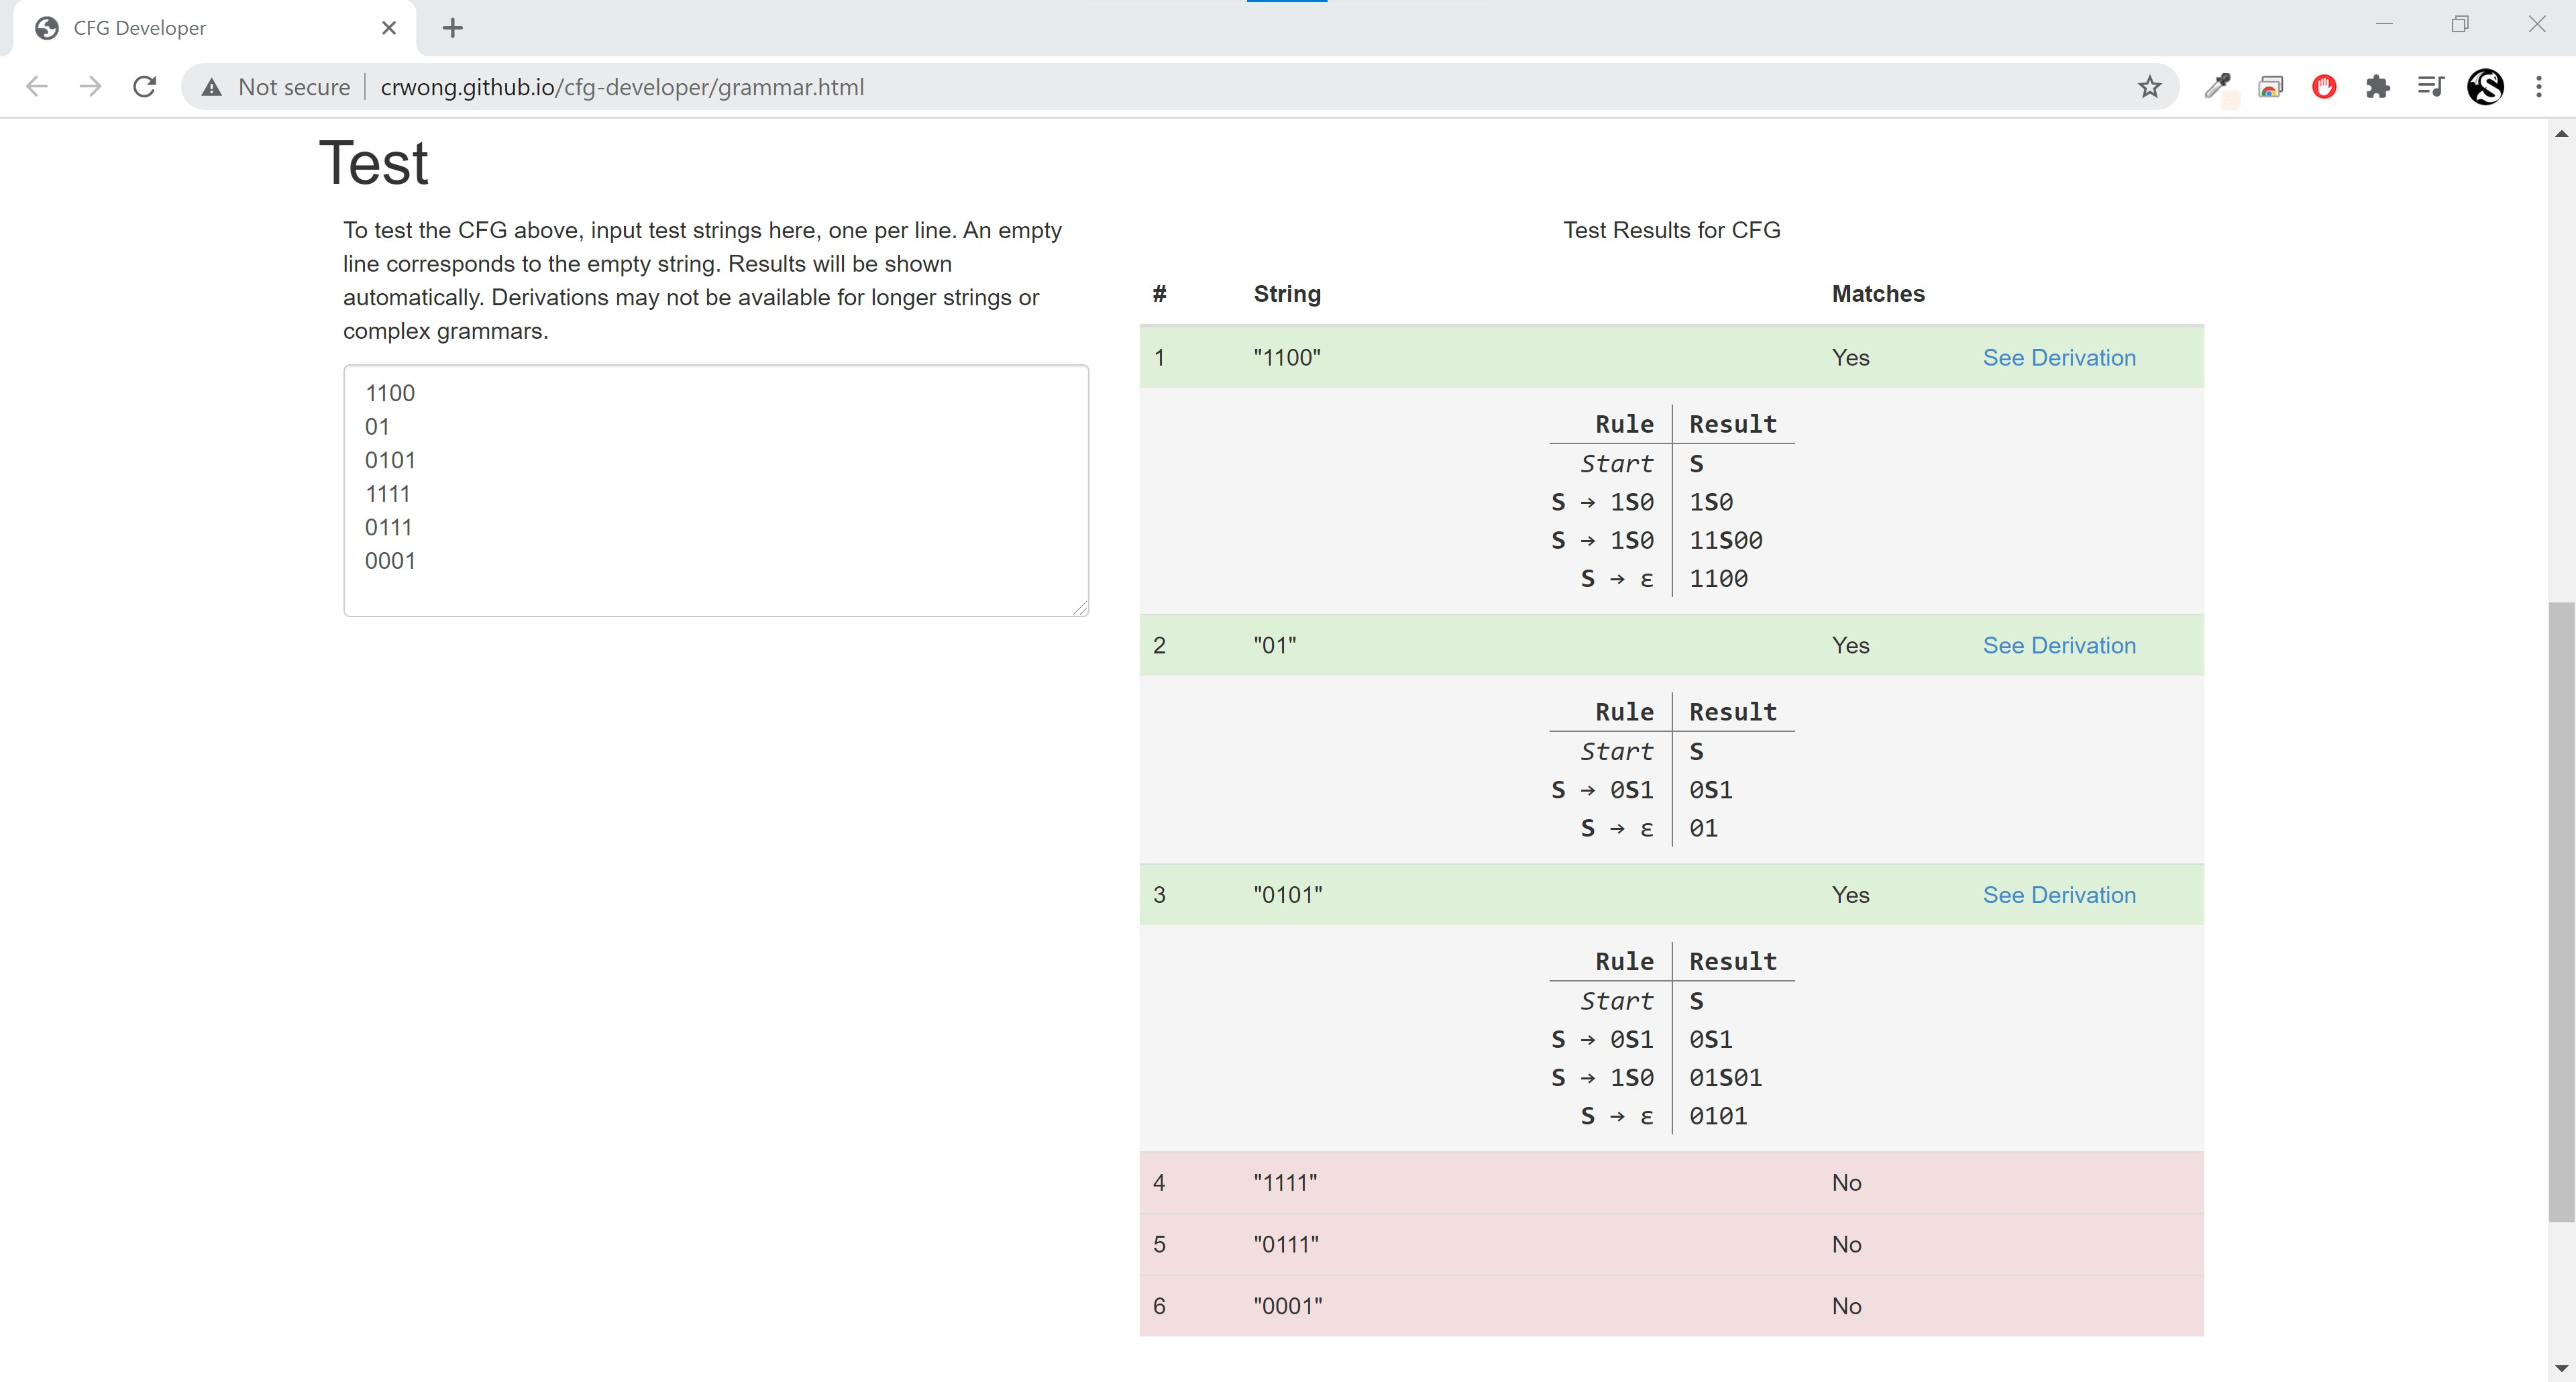
\includegraphics[scale=0.298]{images/L6.jpg}
    \end{center}
  \end{problem}

  \begin{problem}{5.1}
    \begin{center}
      \begin{tikzpicture}[>=stealth',shorten >=1pt,auto,node distance=3cm]
        \node[state, initial] (q0) {$q_0$};
        \node[state] (q1) [right of = q0] {$q_1$};
        \node[state, accepting] (q2) [right of = q1] {$q_2$};

        \path[->] (q0) edge[loop above] node {$
          \begin{matrix}
            a, \epsilon &\to & a\\
            close, \epsilon &\to & close\\
            \times, \epsilon &\to & \times\\
            +, \epsilon &\to & +\\
            -, \epsilon &\to & -\\
            \div, \epsilon &\to & \div\\
            open, \epsilon &\to & open
          \end{matrix}
        $} (q0);

        \path[->] (q0) edge node {$\epsilon, \Sigma \to \epsilon$} (q1);
        \path[->] (q1) edge node {$\epsilon, Z_0 \to \epsilon$} (q2);
      \end{tikzpicture}
    \end{center}
  \end{problem}

  \begin{problem}{5.2}
    \begin{center}
      \begin{tikzpicture}[>=stealth',shorten >=1pt,auto,node distance=3cm]
        \node[state, initial] (q0) {$q_0$};
        \node[state] (q1) [right of = q0] {$q_1$};
        \node[state, accepting] (q2) [right of = q1] {$q_2$};

        \path[->] (q0) edge[loop above] node {$
          \begin{matrix}
            1, 0 &\to & 10\\
            0, 0 &\to & 00\\
            1, 1 &\to & 11\\
            0, 1 &\to & 01\\
            1, Z_0 &\to & 1 Z_0\\
            0, Z_0 &\to & 0 Z_0
          \end{matrix}
        $} (q0);

        \path[->] (q0) edge node {$\Sigma, \epsilon \to \epsilon$} (q1);
        \path[->] (q1) edge[loop above] node {$
          \begin{matrix}
            1, 1 &\to & \epsilon\\
            0, 0 &\to & \epsilon
          \end{matrix}
        $} (q1);

        \path[->] (q1) edge node {$Z_0, Z_0 \to Z_0$} (q2);
      \end{tikzpicture}
    \end{center}
  \end{problem}

  \begin{problem}{5.3}
    \begin{center}
      \begin{tikzpicture}[>=stealth',shorten >=1pt,auto,node distance=3cm]
        \node[state, initial] (q0) {$q_0$};
        \node[state] (q1) [right of = q0] {$q_1$};
        \node[state, accepting] (q2) [right of = q1] {$q_2$};

        \path[->] (q0) edge node {$\epsilon, Z_0 \to \Sigma Z_0$} (q1);
        
        \path[->] (q1) edge[loop above] node {$
          \begin{matrix}
            1, 1 &\to & \epsilon\\
            0, 0 &\to & \epsilon
          \end{matrix}
        $} (q2);

        \path[->] (q1) edge node {$\epsilon, Z_0 \to \epsilon$} (q2);
      \end{tikzpicture}
    \end{center}
  \end{problem}
\end{document}